For this part, we implemented the Direct Linear Transform (DLT) method and tested it on the synthetic data and the slide/frame image pair data from assignment 9. For the synthetic data, we randomly generated 4, 5, and 6 pairs of $(x, y)$ coordinates, twice: one as "actual" points and one as the "estimate" or the point match. We did this $10$ times and yield the RMS errors as shown in Table~\ref{table:rms} below. It's a little difficult to tell if the code is working since the errors stay between (0.3, 0.4) (range tested through trial-and-error) for any number of pairs. We conclude that since we only need 4 good matches, the number of pairs is not making much of a difference in the homography found using the DLT method.

\begin{table}[h]
\begin{center}
\begin{tabular}{|c|c|c|c|c|}
\hline
Number of Pairs & RMS  \\
\hline
4 & 0.3108 \\
\hline
5 & 0.3235 \\
\hline
6 & 0.3267 \\ 
\hline
\end{tabular}
\end{center}
\caption{ RMS error of the transformation for 4, 5, and 6 randomly generated pairs of $(x, y)$-coordinates lying between a $[0,1]\times[0,1]$ window.}
\label{table:rms}
\end{table}

Moving on to the slide/frame image pairs, we collected 8 distinct points using mouse clicks as shown in Fig.~\ref{fig:slideframe} for all three slide/frame pairs. Then using 4 of these clicked points, we computed the homography using the DLT method for each slide/frame pair. Using this homography, we estimated the corresponding slide coordinates to the points on the video frame image. The Fig.~\ref{fig:slideframe_est} shows the visualization on the video frame images, displaying the 8 clicked points in red and the 8 mapped locations in yellow. {\it Please note: previously, we had issue with DLT due to which the estimated (yellow) points were shifted. This issue occured because of two things: 1) we were rescaling the points to [0, 1], and 2) we forgot to normalize the homogenous coordinates so that the last column had all 1s.}

\clearpage
\begin{figure}[ht]
	\begin{subfigure}{0.5\textwidth}
	    {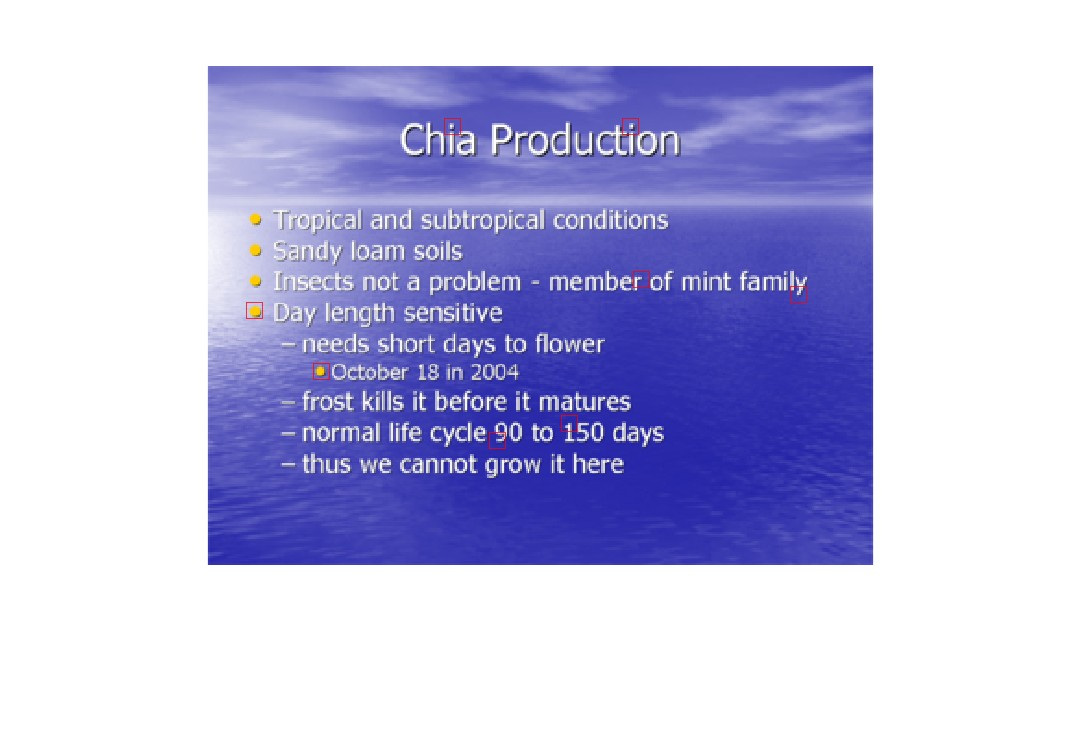
\includegraphics[width=3in]{figs/vizSlidePts_1.jpg}}
		\caption{Slide 1}
	\end{subfigure}
	\begin{subfigure}{0.5\textwidth}
	    {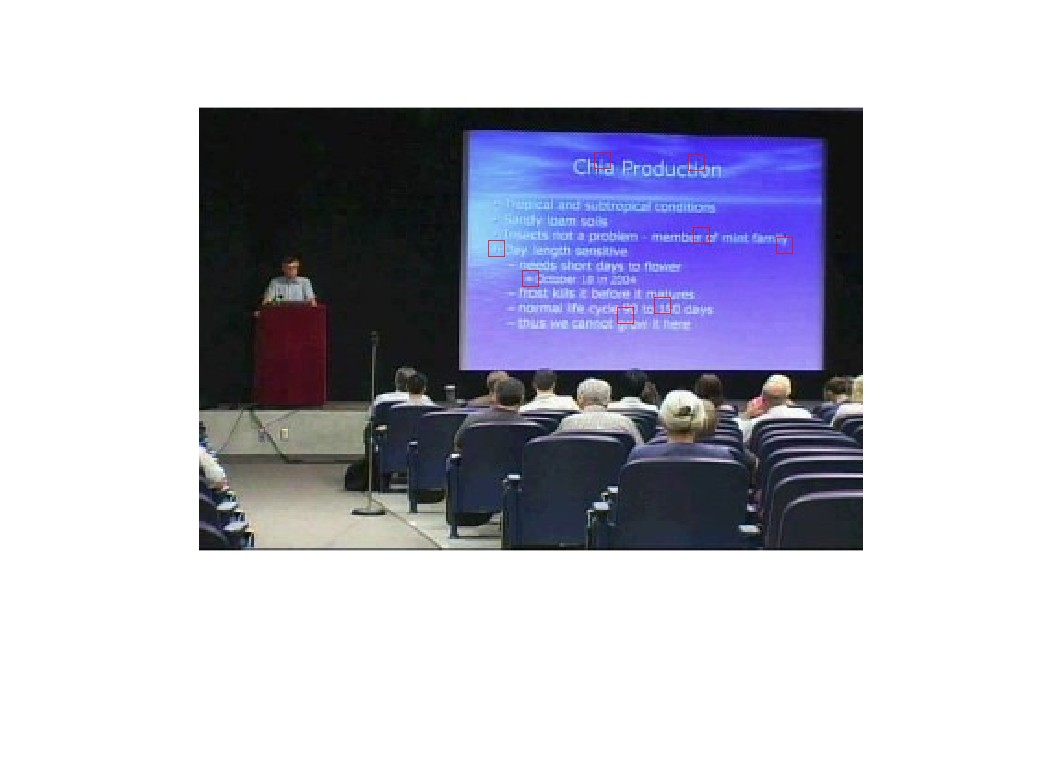
\includegraphics[width=3in]{figs/vizFramePts_1.jpg}}
		\caption{Frame 1}
	\end{subfigure}
	\begin{subfigure}{0.5\textwidth}
	    {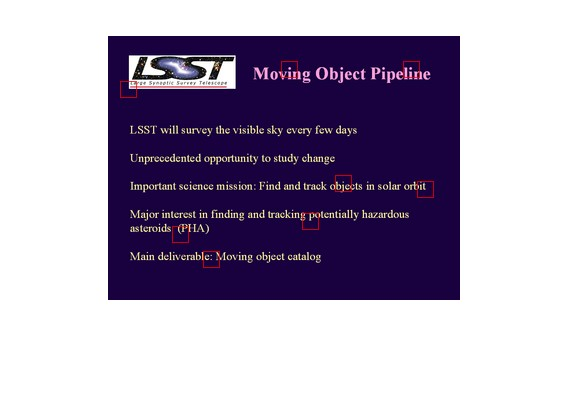
\includegraphics[width=3in]{figs/vizSlidePts_2.jpg}}
		\caption{Slide 2}
	\end{subfigure}
	\begin{subfigure}{0.5\textwidth}
	    {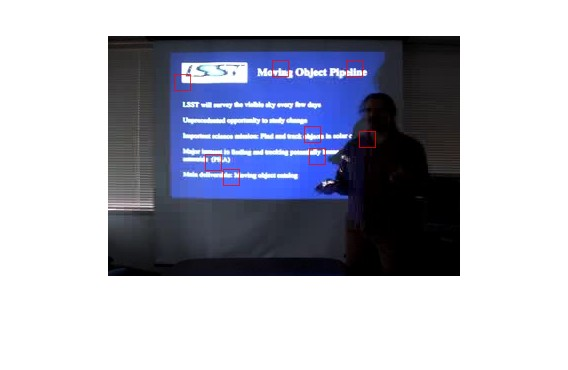
\includegraphics[width=3in]{figs/vizFramePts_2.jpg}}
		\caption{Frame 2}
	\end{subfigure}
	\begin{subfigure}{0.5\textwidth}
	    {
\includegraphics[width=3in]{figs/vizSlidePts_3.jpg}}
		\caption{Slide 3}
	\end{subfigure}
	\begin{subfigure}{0.5\textwidth}
	    {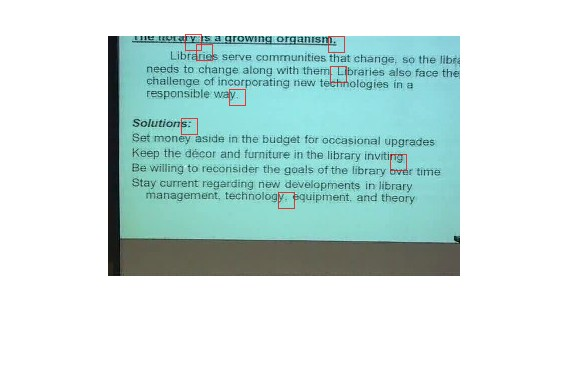
\includegraphics[width=3in]{figs/vizFramePts_3.jpg}}
	    \caption{Frame 3}
	\end{subfigure}
	\caption{Figure showing collected 8 matching points using manual mouse clicking. The points were chosen by focusing on distinct locations that were least ambiguous.}
	\label{fig:slideframe}
\end{figure}

\clearpage
\begin{figure}[ht]
	\begin{subfigure}{0.4\textwidth}
	    {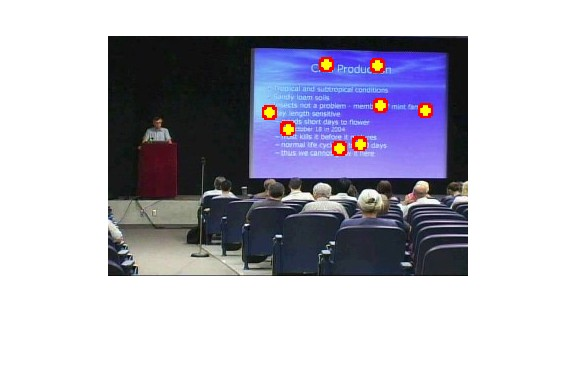
\includegraphics[width=3in]{new_figs/fBSF1.jpg}}
		\caption{Estimated points for Frame 1}
	\end{subfigure}
	\begin{subfigure}{0.4\textwidth}
	    {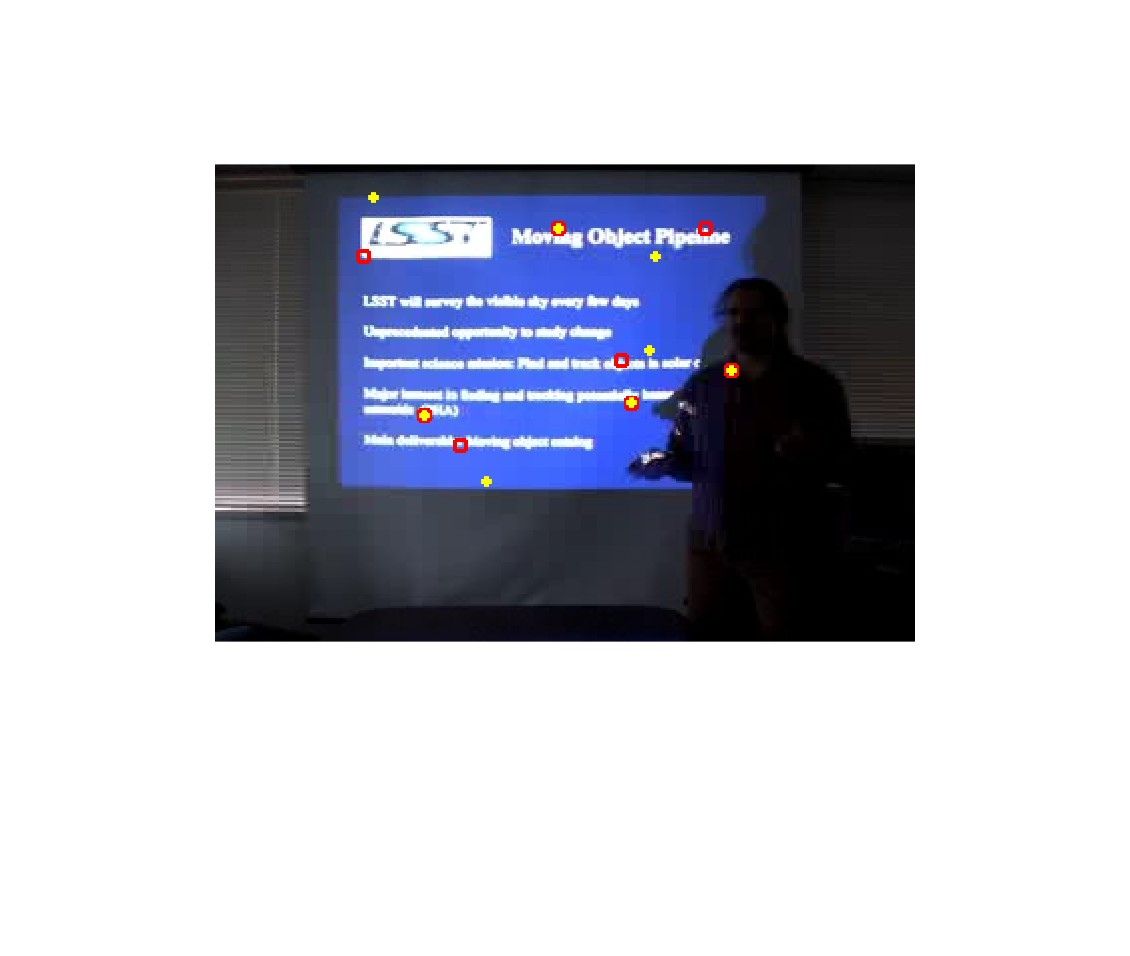
\includegraphics[width=3in]{new_figs/fBSF2.jpg}}
		\caption{Estimated points for Frame 2}
	\end{subfigure}
	\begin{subfigure}{0.4\textwidth}
	    {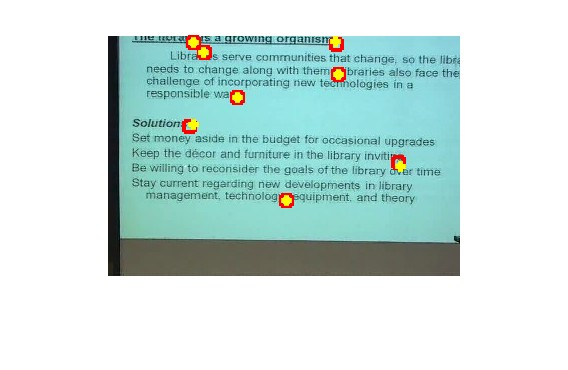
\includegraphics[width=3in]{new_figs/fBSF3.jpg}}
		\caption{Estimated points for Frame 3}
	\end{subfigure}
	\caption{Figure showing the clicked points (in red) against the estimated points computed using homography (in yellow). Note that the subset of points chosen to compute the homography have a visible overlap (that is, yellow marker is perfectly contained in the red square).}
	\label{fig:slideframe_est}
\end{figure}

% RMS errors yielded for each pair are shown in Table~\ref{table:rmssf}
% \begin{table}[h]
% \begin{center}
% \begin{tabular}{|c|c|c|c|c|}
% \hline
% Slide/Frame Pair & RMS  \\
% \hline
% Slide/Frame 1 & 0.1750 \\
% \hline
% Slide/Frame 2 & 0.1756 \\
% \hline
% Slide/Frame 3 & 0.1947 \\ 
% \hline
% \end{tabular}
% \end{center}
% \caption{ RMS error of the difference between the clicked points and the estimated points on the video frame images.}
% \label{table:rmssf}
% \end{table}

